\documentclass[12pt,a4paper]{article}
\usepackage[margin=0.85in]{geometry}
\usepackage[T1]{fontenc}
\usepackage{lmodern,microtype,booktabs,longtable,array,enumitem,xcolor,graphicx,tikz,fancyhdr}
\usetikzlibrary{arrows.meta,positioning}
\usepackage[hidelinks]{hyperref}
\usepackage{seqsplit}
\setlength{\emergencystretch}{3em}
\setlength{\headheight}{15pt}
\setlength{\parskip}{5pt}
\setlength{\parindent}{0pt}
\pagestyle{fancy}\fancyhf{}\fancyhead[L]{Group B: GPU sharing review}\fancyhead[R]{Interim evidence checkpoint}\fancyfoot[C]{\thepage}
\begin{document}
\begin{titlepage}\centering
{\large NED University of Engineering and Technology\\Department of Software Engineering\par}\vspace{1.5cm}
{\LARGE\bfseries GPU Sharing for Multi-Tenant Inference\par}\vspace{0.5cm}
{\Large Search, Screening and Extraction Checkpoint\par}\vspace{0.7cm}
{\large Operating Systems CEP, Topic 23\\Work through guideline Section 14\par}\vspace{1cm}
Eshaal Faisal\\Raazia Imran Reshamwala\\Rameen Siddiqui\vspace{1cm}
\begin{quote}Status: interim research evidence. Selection, independent review and final inclusion remain open. The submitted 27 September 2026 protocol is preserved.\end{quote}
\vfill 15 October 2026
\end{titlepage}
\tableofcontents\newpage

\section{Purpose and engineering problem}
This checkpoint continues Group B's submitted protocol toward guideline Sections 7-14. The decision concerns how one physical GPU can support concurrent inference tenants through time-slicing, MPS, MIG and API interception/remoting while balancing utilization, latency and isolation. Multi-GPU papers qualify only when a within-device inference-sharing result is separable. This report documents actual imported data and bounded source checks; it does not claim a completed systematic review.


The review method follows software-engineering SLR guidance and transparent PRISMA reporting \cite{kitchenham,prisma,prismas}.
\section{Research questions}
\begin{longtable}{p{0.08\linewidth}p{0.84\linewidth}}
\toprule
RQ & Preserved focus\\\midrule
\endhead
RQ1 & Mechanism families, sharing granularity, implementation layer and isolation boundary.\\
RQ2 & Metric definitions and comparability of hardware, workload, baselines and methods.\\
RQ3 & Conditions under which utilization, throughput, density and latency change.\\
RQ4 & Resource/fault isolation, implementation costs, trade-offs and conflicting evidence.\\
RQ5 & Conditional engineering choices, confidence and alternatives.\\
\bottomrule
\end{longtable}

\section{Sources and shared-data provenance}
The user explicitly authorized reuse of Group A's searches and findings with attribution. We imported its committed IEEE/Springer metadata and preserved its assessments as prior assessments. Group B does not claim to have re-executed those searches. Group A source snapshot: adf4a1e827f71610eba21785fbf5cbac8793fbfc. The shared materials remain under evidence/imports/group-a. ACM bibliography exports supplied through Drive remain untouched under evidence/imports/acm. The import manifest records SHA-256 hashes and counts.


\begin{longtable}{p{0.15\linewidth}p{0.14\linewidth}p{0.62\linewidth}}
\toprule
Source & Rows & Evidence status\\\midrule
\endhead
ACM & 1582 & 79 original BibTeX files; exact query-to-batch mapping unresolved\\
Springer & 587 & Group A master search; broad full-text indexed scope\\
IEEE & 102 & Group A executed metadata capture; five-run shared log includes four IEEE runs\\
Other sources & 20 & 20 selected shared leads; not a systematic citation census\\
\bottomrule
\end{longtable}

Database occurrences total 2,271. The 20 supplementary leads are a separate route, giving 2,291 total imported occurrences. These counts are export/capture counts, not a claim that ACM displayed exactly 1,582 hits. ScienceDirect's earlier 100 incoming RIS occurrences remain preserved separately and are excluded from this active checkpoint by the user's instruction. No source was deleted.


\section{Search strategy and deviations}
Group B's submitted protocol specifies 12 main-window expressions and four older-MPS expressions. The imported Group A search design uses a different master/family vocabulary and broad Springer field. Reuse saves collection effort but does not establish equivalence to every Group B planned query. Appendix A preserves the exact shared executed expressions and settings. The ACM files do not establish their original query, field, date filters, displayed hits or pagination. Those unknowns remain unknown.


\begin{longtable}{p{0.19\linewidth}p{0.13\linewidth}p{0.59\linewidth}}
\toprule
Run & Shared count & Field and coverage\\\midrule
\endhead
IEEE-MPS & 25 & All metadata (Search by All); not field-qualified Command Search; Publication years2020-2026; date/language/type checked during screening\\
IEEE-MIG & 23 & All metadata (Search by All); not field-qualified Command Search; Publication years2020-2026; date/language/type checked during screening\\
IEEE-TEMPORAL & 45 & All metadata (Search by All); not field-qualified Command Search; Publication years2020-2026; date/language/type checked during screening\\
IEEE-API & 9 & All metadata (Search by All); not field-qualified Command Search; Publication years2020-2026; date/language/type checked during screening\\
SPR-MASTER & 587 & General search/full-text indexed collection; English; Research article OR Conference paper;2020-2026; manual cutoff\\
\bottomrule
\end{longtable}

Search-coverage gaps: ACM run mapping and completeness; missing prespecified older-MPS lanes; unexecuted Group B expressions; broad Springer body-search noise; ScienceDirect deferred. The shared search cutoff is 11 October 2026; ACM export upload/modified times cannot substitute for search timestamps. Publication-date eligibility for ACM candidates must use the documented actual run date, or a clearly adopted and recorded common cutoff.


\section{Eligibility and screening rules}
\begin{longtable}{p{0.16\linewidth}p{0.76\linewidth}}
\toprule
Criterion & Operational rule\\\midrule
\endhead
IC1 & Final English peer-reviewed full journal or conference primary study.\\
IC2-IC3 & Distinct concurrent tenants share one physical GPU through an assigned mechanism, with separable inference evidence.\\
IC4-IC5 & Inspectable relevant outcome and sufficient methods/configuration; separable local result permitted in larger systems.\\
IC6 & Main date window or individually justified older seminal exception.\\
EC1 & Non-primary/non-peer-reviewed, survey, poster, abstract-only or container item.\\
EC2-EC5 & Training-only/no concurrent inference; hardware-only; aggregate cluster-only; non-GPU-only.\\
EC6-EC7 & Insufficient assessed full-text detail; outside date/language criteria.\\
\bottomrule
\end{longtable}

Missing full text is a retrieval status, not EC6. Title uncertainty is retained. Multiple reports are linked to a study rather than counted as separate studies. The existing REEF conference/journal versions require a preferred-report decision. Original independent votes must be preserved; there is currently one Group B AI reviewer, not two human reviewers.


\section{Duplicate linkage and payload}
Deterministic linkage identifies 44 repeated occurrences, leaving 2247 canonical records for review. The keys use normalized DOI or exact publisher URL; identifier-free ACM copies additionally require identical normalized title, authors and year. Different DOIs are not silently collapsed. There are 41 title-match pairs still requiring identity/version review. These are not removed from the active counts.


The earlier pasted checkpoint reported 74 duplicates and 2,217 records. Those figures were not recovered as a committed row-level log. This reconstruction deliberately reports its own reproducible result instead of repeating an unverified total. Identity linkage remains subject to review of the 41 pairs. The imported ACM payload also contains 609 proceedings containers, seven books and one technical report; these explain many low-relevance hits and require distinct EC1 recommendations.


\section{Current screening results}
\begin{longtable}{p{0.57\linewidth}p{0.34\linewidth}}
\toprule
Measure & Observed state\\\midrule
\endhead
Canonical records & 2247\\
Recorded first-review decisions & 800\\
Exclude recommendations & 652\\
Retain/uncertain recommendations & 148\\
Awaiting first review & 1447\\
Independent second-review and final decisions & Pending\\
Source-checked priority reports & 5\\
Final included primary-study count & Not established\\
\bottomrule
\end{longtable}

The 800 first-review rows comprise 183 individually inspected high-priority titles and 617 explicit BibTeX container/book/report type checks. Recommendations are preliminary, with abstract verification where needed and independent checking still open. The remaining triage labels are automated prioritization signals, not exclusion decisions. No 1,813-record automated triage category is reported as a final exclusion.


\section{Interim PRISMA 2020 accounting}
The following diagram is a pending-stage accounting view using PRISMA categories, not a completed official PRISMA result. Final screening, reports sought/not retrieved, assessed exclusions and included-study totals require resolved record/report/study links and independent review. Four targeted backward-reference links are logged separately; three are unimported candidate leads and do not inflate current identification counts.


\begin{center}
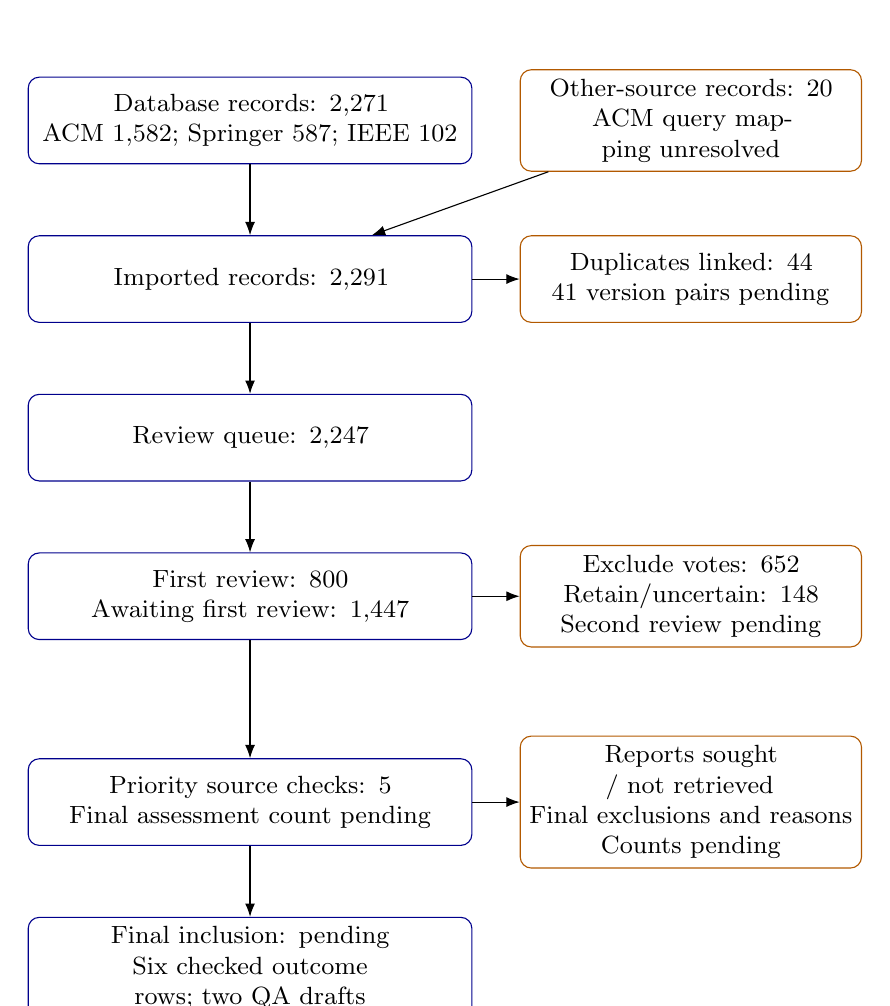
\begin{tikzpicture}[box/.style={draw=blue!55!black,rounded corners,align=center,text width=5.4cm,minimum height=1.1cm,font=\small},side/.style={box,draw=orange!70!black,text width=4.1cm},>=Latex,node distance=0.9cm]
\node[box] (db) {Database records: 2,271\\ACM 1,582; Springer 587; IEEE 102};
\node[side,right=0.6cm of db] (other) {Other-source records: 20\\ACM query mapping unresolved};
\node[box,below=of db] (all) {Imported records: 2,291};
\node[side,right=0.6cm of all] (dup) {Duplicates linked: 44\\41 version pairs pending};
\node[box,below=of all] (queue) {Review queue: 2,247};
\node[box,below=of queue] (first) {First review: 800\\Awaiting first review: 1,447};
\node[side,right=0.6cm of first] (votes) {Exclude votes: 652\\Retain/uncertain: 148\\Second review pending};
\node[box,below=1.5cm of first] (ft) {Priority source checks: 5\\Final assessment count pending};
\node[side,right=0.6cm of ft] (retr) {Reports sought / not retrieved\\Final exclusions and reasons\\Counts pending};
\node[box,below=of ft] (inc) {Final inclusion: pending\\Six checked outcome rows; two QA drafts};
\draw[->] (db)--(all);\draw[->] (other)--(all);\draw[->] (all)--(queue);\draw[->] (all)--(dup);\draw[->] (queue)--(first);\draw[->] (first)--(votes);\draw[->] (first)--(ft);\draw[->] (ft)--(retr);\draw[->] (ft)--(inc);
\end{tikzpicture}
\end{center}

\section{Citation chasing}
A targeted backward pilot inspected four references from gpulets: Prophet [4], Baymax [5], Clipper [15] and GSLICE [17], on printed pages 210-211. GSLICE already occurs in the imported payload. The other three are candidate leads awaiting metadata/full-text eligibility checks; their older dates require individual justification if retained. This is a four-reference pilot, not exhaustive backward/forward snowballing. The remaining references and forward citations remain to be searched and logged.


\section{Priority full-text checks}
\begin{longtable}{p{0.16\linewidth}p{0.76\linewidth}}
\toprule
Report & Group B first-review finding\\\midrule
\endhead
VastPipe & Local A100 inference model pairs use tuned/default/no MPS; local GPU outcomes are separable from NPU cluster results. Remaining: Original chart check, second reviewer, exact quotas/batches, all source sections. Source: pp457-459, sections6.7-6.9, Figs14-16\\
iGniter & Four inference models co-located on one V100, MPS quotas and local latency prediction are explicit; fleet costs kept distinct. Remaining: Second reviewer; OS/driver extraction; full-source verification of remaining fields. Source: pp820-824, sections4.2,5.1-5.4, Figs13-17\\
gpulets & One-device paired inference interference and MPS partitioning are separable from multi-GPU scheduler results. Remaining: Second reviewer, complete outcome extraction and QA. Source: pp201-203,207; sections2,3,5.1; Figs4,7; Tables2-3\\
PipeSwitch & Separable inference latency under local training/inference co-location; temporal switching and MPS comparator. Remaining: Second reviewer; mixed training/inference scope sensitivity; complete QA. Source: pp508-509, section6.1, Tables3-4\\
REEF conference & Concurrent RT/BE inference tenants on MI50; later journal report must be linked as the same study. Remaining: Verify journal equivalence before preferred-report choice; second reviewer; no double counting. Source: p548 section7.1 Table2; pp539-542\\
\bottomrule
\end{longtable}

\section{Quality appraisal and calibration}
Group A's ten-item 0-1 scale has different criterion meanings from Group B's submitted Q1-Q10 0-2 rubric. Multiplying the totals would be invalid. Two fresh first-review appraisals are recorded with rationale and source anchors; the second reviewer and reconciliation columns remain blank. N/A is used only for an outcome claim genuinely outside the bounded evidence being appraised. The VastPipe appraisal is explicitly restricted to its local GPU evidence, not the NPU experiments.


\begin{longtable}{p{0.2\linewidth}p{0.22\linewidth}p{0.22\linewidth}p{0.18\linewidth}}
\toprule
Report & First-review sum & Applicable max & Normalized\\\midrule
\endhead
GB-P001 & 13.0 & 18 & 72.2\%\\
GB-P002 & 17.0 & 20 & 85.0\%\\
\bottomrule
\end{longtable}

Scores do not establish final inclusion, nor do they replace the source check. No final synthesis sensitivity conclusion is yet supported. Each appraisal retains ten separate criterion rows so the team can challenge a score without losing its original rationale.


\section{Data extraction through guideline Section 14}
The active register contains six newly checked outcomes across four priority reports. Five older pilot rows remain in evidence/pilot/extraction.csv with their original manuscript/version caveats. They are not added to final included-study counts. The full extraction category specification A-M remains in the submitted protocol. Use not-extracted for fields not yet transcribed, NR only when the source was checked and does not report the item, and an empty checker field until an independent check occurs.


\begin{longtable}{p{0.27\linewidth}p{0.65\linewidth}}
\toprule
Report / metric & Checked result and interpretation\\\midrule
\endhead
GB-P001 / Throughput ratio & 2.7 x; NVIDIA A100; VGG16+GoogLeNet. Baseline: No MPS. Anchor: pp457-458 Fig14 and accompanying prose. Batch/rate/quotas unresolved; not tail-latency evidence\\
GB-P001 / Throughput ratio & 1.5 x; NVIDIA A100; VGG16+GoogLeNet. Baseline: Default MPS. Anchor: pp457-458 Fig14 and accompanying prose. Same comparison family; not a universal average\\
GB-P002 / Prediction error range & 1.53-5.02 percent; NVIDIA V100; AlexNet/ResNet50/VGG19/SSD; batch3. Baseline: Measured local latency. Anchor: p822 section5.2 Fig13. Prediction accuracy, not utilization or latency speedup\\
GB-P002 / Initial p99 latency & 15.6 ms; NVIDIA V100; W1 with W5 and W11. Baseline: W1 latency SLO10ms. Anchor: p823 section5.3 Fig17 prose. Transient violation precedes recovery; no unconditional guarantee\\
GB-P004 / Additional end-to-end latency & 6.01 ms; NVIDIA V10016GB; ResNet152 inference batch8 + training batch32. Baseline: Ready-model latency subtracted; MPS overhead307.02ms. Anchor: p509 Table3; setup p508 section6. Mean100 runs; overhead, not total latency or p99; MPS uses unified-memory swapping\\
GB-P003 / Distribution threshold:90\% of measured pairs & 17.66 percent overhead below threshold; RTX2080Ti11GB; Paired model inferences. Baseline: Solo-running latency. Anchor: p203 Fig7. Across-pair CDF, not request-p90/p99; no hostile-memory/fault test\\
\bottomrule
\end{longtable}

Checked source reports are VastPipe, iGniter, gpulets and PipeSwitch \cite{vastpipe,igniter,gpulets,pipeswitch}. REEF\textquotesingle s conference report has a bounded configuration check \cite{reef}; a later journal extension is already a shared version lead.
\section{Interpretation limits}
The extracted quantities are deliberately kept distinct. Prediction error is not a utilization gain. A p99 recovery example does not prove an unconditional SLO guarantee. Additional end-to-end latency is not total response time. A CDF across model-pair overheads is not a request-latency percentile. Fleet cost/GPU-count benefits cannot be attributed to local GPU utilization without a valid denominator. Performance interference does not prove memory, security or fault containment.


\section{Work to close before submission}
\begin{longtable}{p{0.27\linewidth}p{0.65\linewidth}}
\toprule
Owner / task & Concrete output\\\midrule
\endhead
Eshaal: source and abstract review & Recover ACM query-to-file mapping from search history/screenshots: exact strings, field, date, hit count and exported pages. Then review assigned screening rows without seeing first-review votes initially.\\
Rameen: priority paper checks & Independently check the five priority reports, six outcomes and 20 QA items. Enter own vote/score and exact page/table. Check the remaining 21 shared candidates in priority order.\\
Raazia / AI: registers and report & Resolve version pairs, continue abstracts and full texts, complete citation chasing, reconcile PRISMA and rebuild report/workbook from the same logs.\\
\bottomrule
\end{longtable}

Measured progress: 800/2247 (35.6\%) canonical records have a first-review recommendation. Five reports have bounded source checks; two have first-review appraisals. Final protocol-compliant screening and inclusion are pending. These are activity-specific measures, not a claim of 50\% or 100\% overall completion. The final CEP additionally needs Sections 15-22: taxonomy, comparison, trade-offs, conflicts, synthesis, recommendation, gaps and limitations.


\appendix\section{Exact imported Group A executed searches}
\subsection{IEEE-MPS}
Database: IEEE Xplore. Date: 2026-10-11; time UTC: not\_recorded. Reviewer/operator: AI-CODEX. Collection: Xplore all metadata.


{\small\ttfamily\raggedright (GPU OR "graphics processing unit") AND (inference OR "model serving" OR "deep learning" OR DNN OR LLM) AND (MPS OR "multi-process service")\par}
Field: All metadata (Search by All); not field-qualified Command Search. Filters: Publication years2020-2026; date/language/type checked during screening. Displayed hits: 25. Captured occurrences: 25. Export method: Public rendered-result metadata; all pages captured; publisher CSV requires personal sign-in; BibTeX export timed out.


\subsection{IEEE-MIG}
Database: IEEE Xplore. Date: 2026-10-11; time UTC: not\_recorded. Reviewer/operator: AI-CODEX. Collection: Xplore all metadata.


{\small\ttfamily\raggedright (GPU OR "graphics processing unit") AND (inference OR "model serving" OR "deep learning" OR DNN OR LLM) AND (MIG OR "multi-instance GPU" OR "GPU partitioning")\par}
Field: All metadata (Search by All); not field-qualified Command Search. Filters: Publication years2020-2026; date/language/type checked during screening. Displayed hits: 23. Captured occurrences: 23. Export method: Public rendered-result metadata; all pages captured; publisher CSV requires personal sign-in; BibTeX export timed out.


\subsection{IEEE-TEMPORAL}
Database: IEEE Xplore. Date: 2026-10-11; time UTC: not\_recorded. Reviewer/operator: AI-CODEX. Collection: Xplore all metadata.


{\small\ttfamily\raggedright (GPU OR "graphics processing unit") AND (inference OR "model serving" OR "deep learning" OR DNN OR LLM) AND ("time slicing" OR "time sharing" OR "context switching")\par}
Field: All metadata (Search by All); not field-qualified Command Search. Filters: Publication years2020-2026; date/language/type checked during screening. Displayed hits: 45. Captured occurrences: 45. Export method: Public rendered-result metadata; all pages captured; publisher CSV requires personal sign-in; BibTeX export timed out.


\subsection{IEEE-API}
Database: IEEE Xplore. Date: 2026-10-11; time UTC: not\_recorded. Reviewer/operator: AI-CODEX. Collection: Xplore all metadata.


{\small\ttfamily\raggedright (GPU OR "graphics processing unit") AND (inference OR "model serving" OR "deep learning" OR DNN OR LLM) AND ("API remoting" OR "CUDA remoting" OR "GPU proxy" OR "GPU virtualization")\par}
Field: All metadata (Search by All); not field-qualified Command Search. Filters: Publication years2020-2026; date/language/type checked during screening. Displayed hits: 9. Captured occurrences: 9. Export method: Public rendered-result metadata; all pages captured; publisher CSV requires personal sign-in; BibTeX export timed out.


\subsection{SPR-MASTER}
Database: Springer Nature Link. Date: 2026-10-11; time UTC: not\_recorded. Reviewer/operator: AI-CODEX. Collection: Springer Nature Link.


{\small\ttfamily\raggedright (GPU OR "graphics processing unit") AND (inference OR "model serving" OR "deep learning" OR DNN OR LLM) AND ("time slicing" OR "time sharing" OR "context switching" OR MPS OR "multi-process service" OR MIG OR "multi-instance GPU" OR "GPU partitioning" OR "API remoting" OR "CUDA remoting" OR "GPU proxy" OR "GPU virtualization")\par}
Field: General search/full-text indexed collection. Filters: English; Research article OR Conference paper;2020-2026; manual cutoff. Displayed hits: 587. Captured occurrences: 587. Export method: Rendered metadata from all30 pages; publisher CSV routes to sign-in.


\section{Evidence-file guide}
\begin{longtable}{p{0.38\linewidth}p{0.54\linewidth}}
\toprule
File & Purpose\\\midrule
\endhead
records.csv & One immutable occurrence per row; source hash and original identity.\\
duplicates.csv / possible\_versions.csv & Resolved deterministic repeats / unresolved title pairs.\\
screening.csv / title\_votes.csv & Editable review queue / preserved first-review events.\\
fulltext\_checks.csv & Five source checks with outstanding criteria/version work.\\
quality.csv / extraction.csv & Fresh Group B first-review appraisal / six outcome records.\\
snowballing.csv & Four backward-reference events; no invented citation census.\\
imports/group-a & Original attributed search data and prior assessments.\\
imports/acm / import\_manifest.csv & Untouched bibliography batches and hash inventory.\\
\bottomrule
\end{longtable}

\section{Audit against instructor headings 1--14}
\begin{longtable}{p{.09\linewidth}p{.24\linewidth}p{.12\linewidth}p{.42\linewidth}}\toprule Heading & Requirement & State & Closure condition\\\midrule\endhead
1 & Background & Prepared & Final evidence-based discussion belongs to final CEP\\
2 & Engineering problem & Prepared & Bound at within-device inference sharing\\
3 & Objective & Prepared & Preserve utilization/latency/isolation focus\\
4 & SLR methodology & Prepared & Executed deviations must remain explicit\\
5 & Required activities / RQs & Prepared & Do not count later synthesis as completed\\
6 & SLR protocol & Prepared & Original preserved; amendments separate\\
7 & Database selection & Partial & ScienceDirect deferred; coverage deviation\\
8 & Search strategy & Partial & ACM mapping and omitted Group B lanes unresolved\\
9 & Literature period & Partial & ACM actual run date/cutoff verification pending\\
10 & Inclusion/exclusion & Partial & 1447 records without first recommendation; independent votes pending\\
11 & PRISMA 2020 & Partial & Final retrieval/eligibility/study counts remain null\\
12 & Search/screening log & Partial & Complete provenance and decisions for every active record\\
13 & Quality assessment & Partial & 2 first-review forms; remaining candidates and independent check pending\\
14 & Data extraction & Partial & 6 fresh outcome rows; complete study form and verification pending\\
\bottomrule\end{longtable}
\section{Completion estimate and immediate handoff}
The measured first-review coverage is 35.6\%. An approximate 40\% readiness estimate is used only for workload planning, not as a verified research-completion percentage or marks prediction. Final eligibility, independent review, completed QA/extraction and final PRISMA remain open.

The full study form is evidence/study\_extraction\_form.csv. It includes software, hardware, tenant mix, batch/load/SLO, baseline, metrics, resource use, scalability, energy, reliability, security, overhead and trade-offs. Missing values are explicitly not-extracted; no zero or not-reported finding is inferred without checking the source.

Raazia with AI maintains records, verifies sources, resolves versions, completes evidence and rebuilds deliverables. Eshaal recovers ACM query/batch provenance and independently reviews screening. Rameen independently checks the five source reports, six outcome rows and two QA forms before extending to remaining shared candidates. Only genuinely independent work is recorded as a second review.
\clearpage\bibliographystyle{ieeetr}\bibliography{references}\end{document}